\begin{frame}{Maillages Quadrilatères et Hexaédriques : Challenges}
    \begin{columns}[T] % align columns
        \begin{column}{.5\textwidth}
            %Un maillage non-structuré pose des problèmes de convergence. \vspace*{.2cm}\\
            \textbf{Qualité du maillage}
            \begin{itemize}
                \item Alignement avec les bords
                \item Angles proche de 90°
                \item Peu de singularités
            \end{itemize}
            
            \textbf{Pas d’algorithme générique}
            \begin{itemize}
                \item Intervention humaine
                \item Subdivision manuelle en blocs structurés
                \item Plusieurs semaines/mois pour construire un maillage
            \end{itemize}
        \end{column}%
        
        \begin{column}{.5\textwidth}
            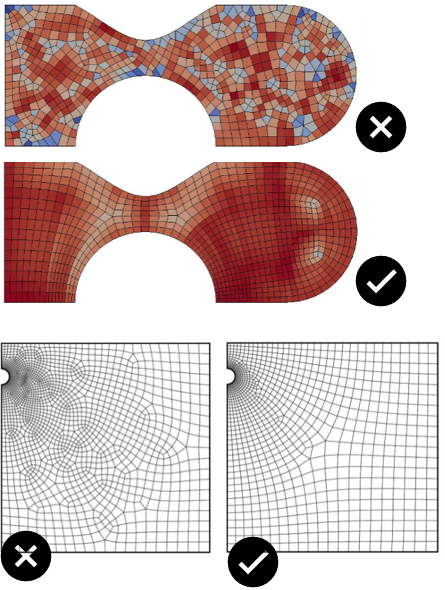
\includegraphics[width=\linewidth]{img/new_images/qualite_maillage_important.PNG}
        \end{column}
    \end{columns}
\end{frame}

\begin{frame}{Objectif de la thèse}
    \centering
    \textbf{Automatiser la génération de maillage quad/hex de haute qualité pour les simulations de grandes déformations}.\\ \vspace{1em}
    \only<1>{ 
        \begin{tabular}{c|c}
            \textit{Entrée} : Maillage tri & \textit{Sortie} : Maillage quad $< 1$ min\\ \hline \\
             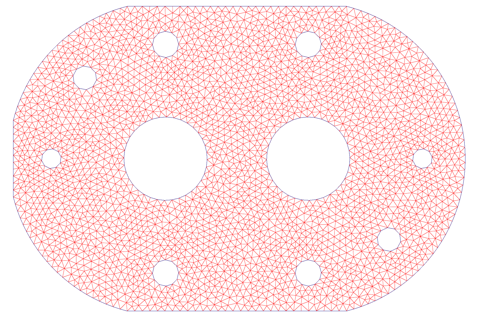
\includegraphics[width=0.45\linewidth]{img/new_images/entree_maillage_tri.png} &  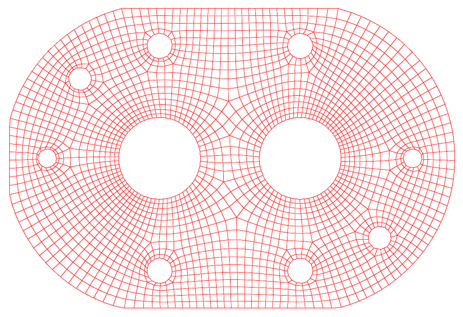
\includegraphics[width=0.45\linewidth]{img/new_images/sortie_maillage_quad.png} \\
        \end{tabular}
    }
    \only<2>{
        \begin{tabular}{c|c}
            \textit{Entrée} : Maillage tétra & \textit{Sortie} : Maillage hex $< 1$ min\\ \hline \\
             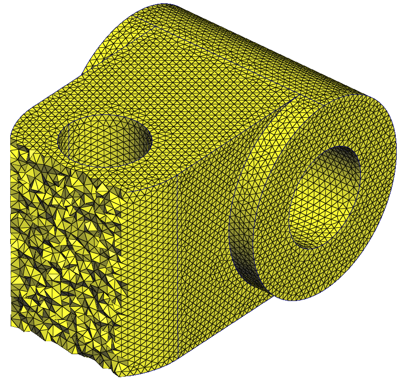
\includegraphics[width=0.4\linewidth]{img/new_images/entree_maillage_tet.png} &  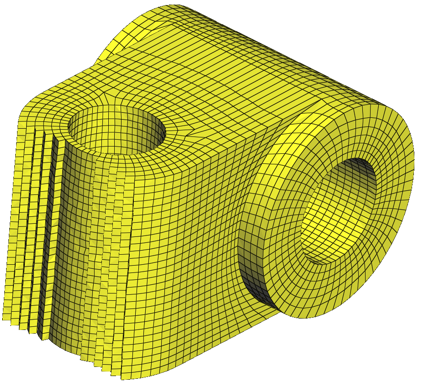
\includegraphics[width=0.4\linewidth]{img/new_images/sortie_maillage_hex.png} \\
        \end{tabular}
    }
    \only<3>{
        \begin{figure}
            \centering
            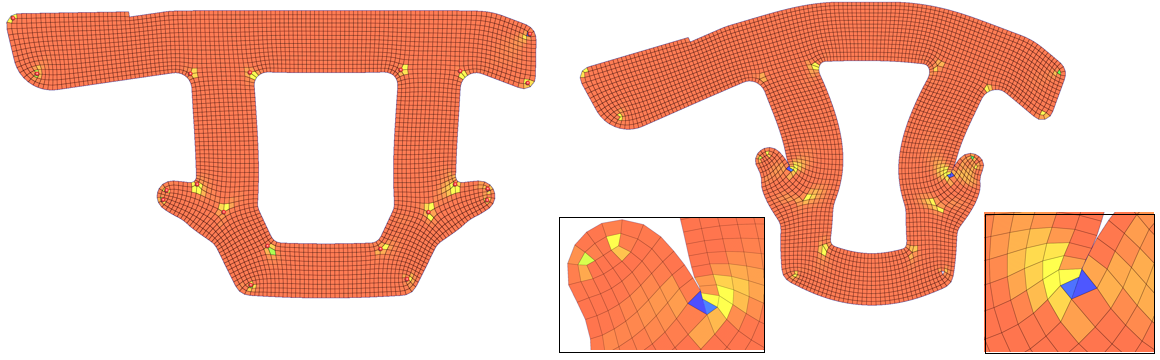
\includegraphics[width=\linewidth]{img/new_images/echec_simu.PNG}
            \caption{Les positions de singularités optimales pour une géométrie initiale peuvent conduire à des quadrilatères de mauvaise qualité après une déformation.}
        \end{figure}
    }
\end{frame}